% TO BE INSERTED INTO ACRONYMS SECTION:

% SSG - symbolic state graph
% CFG - control flow graph
% BB - Basic Block

% tala en highlevel description of implementation, liknande revgen paper section 4.
% https://dslab.epfl.ch/pubs/revgen.pdf

\begin{figure}
    \centering
    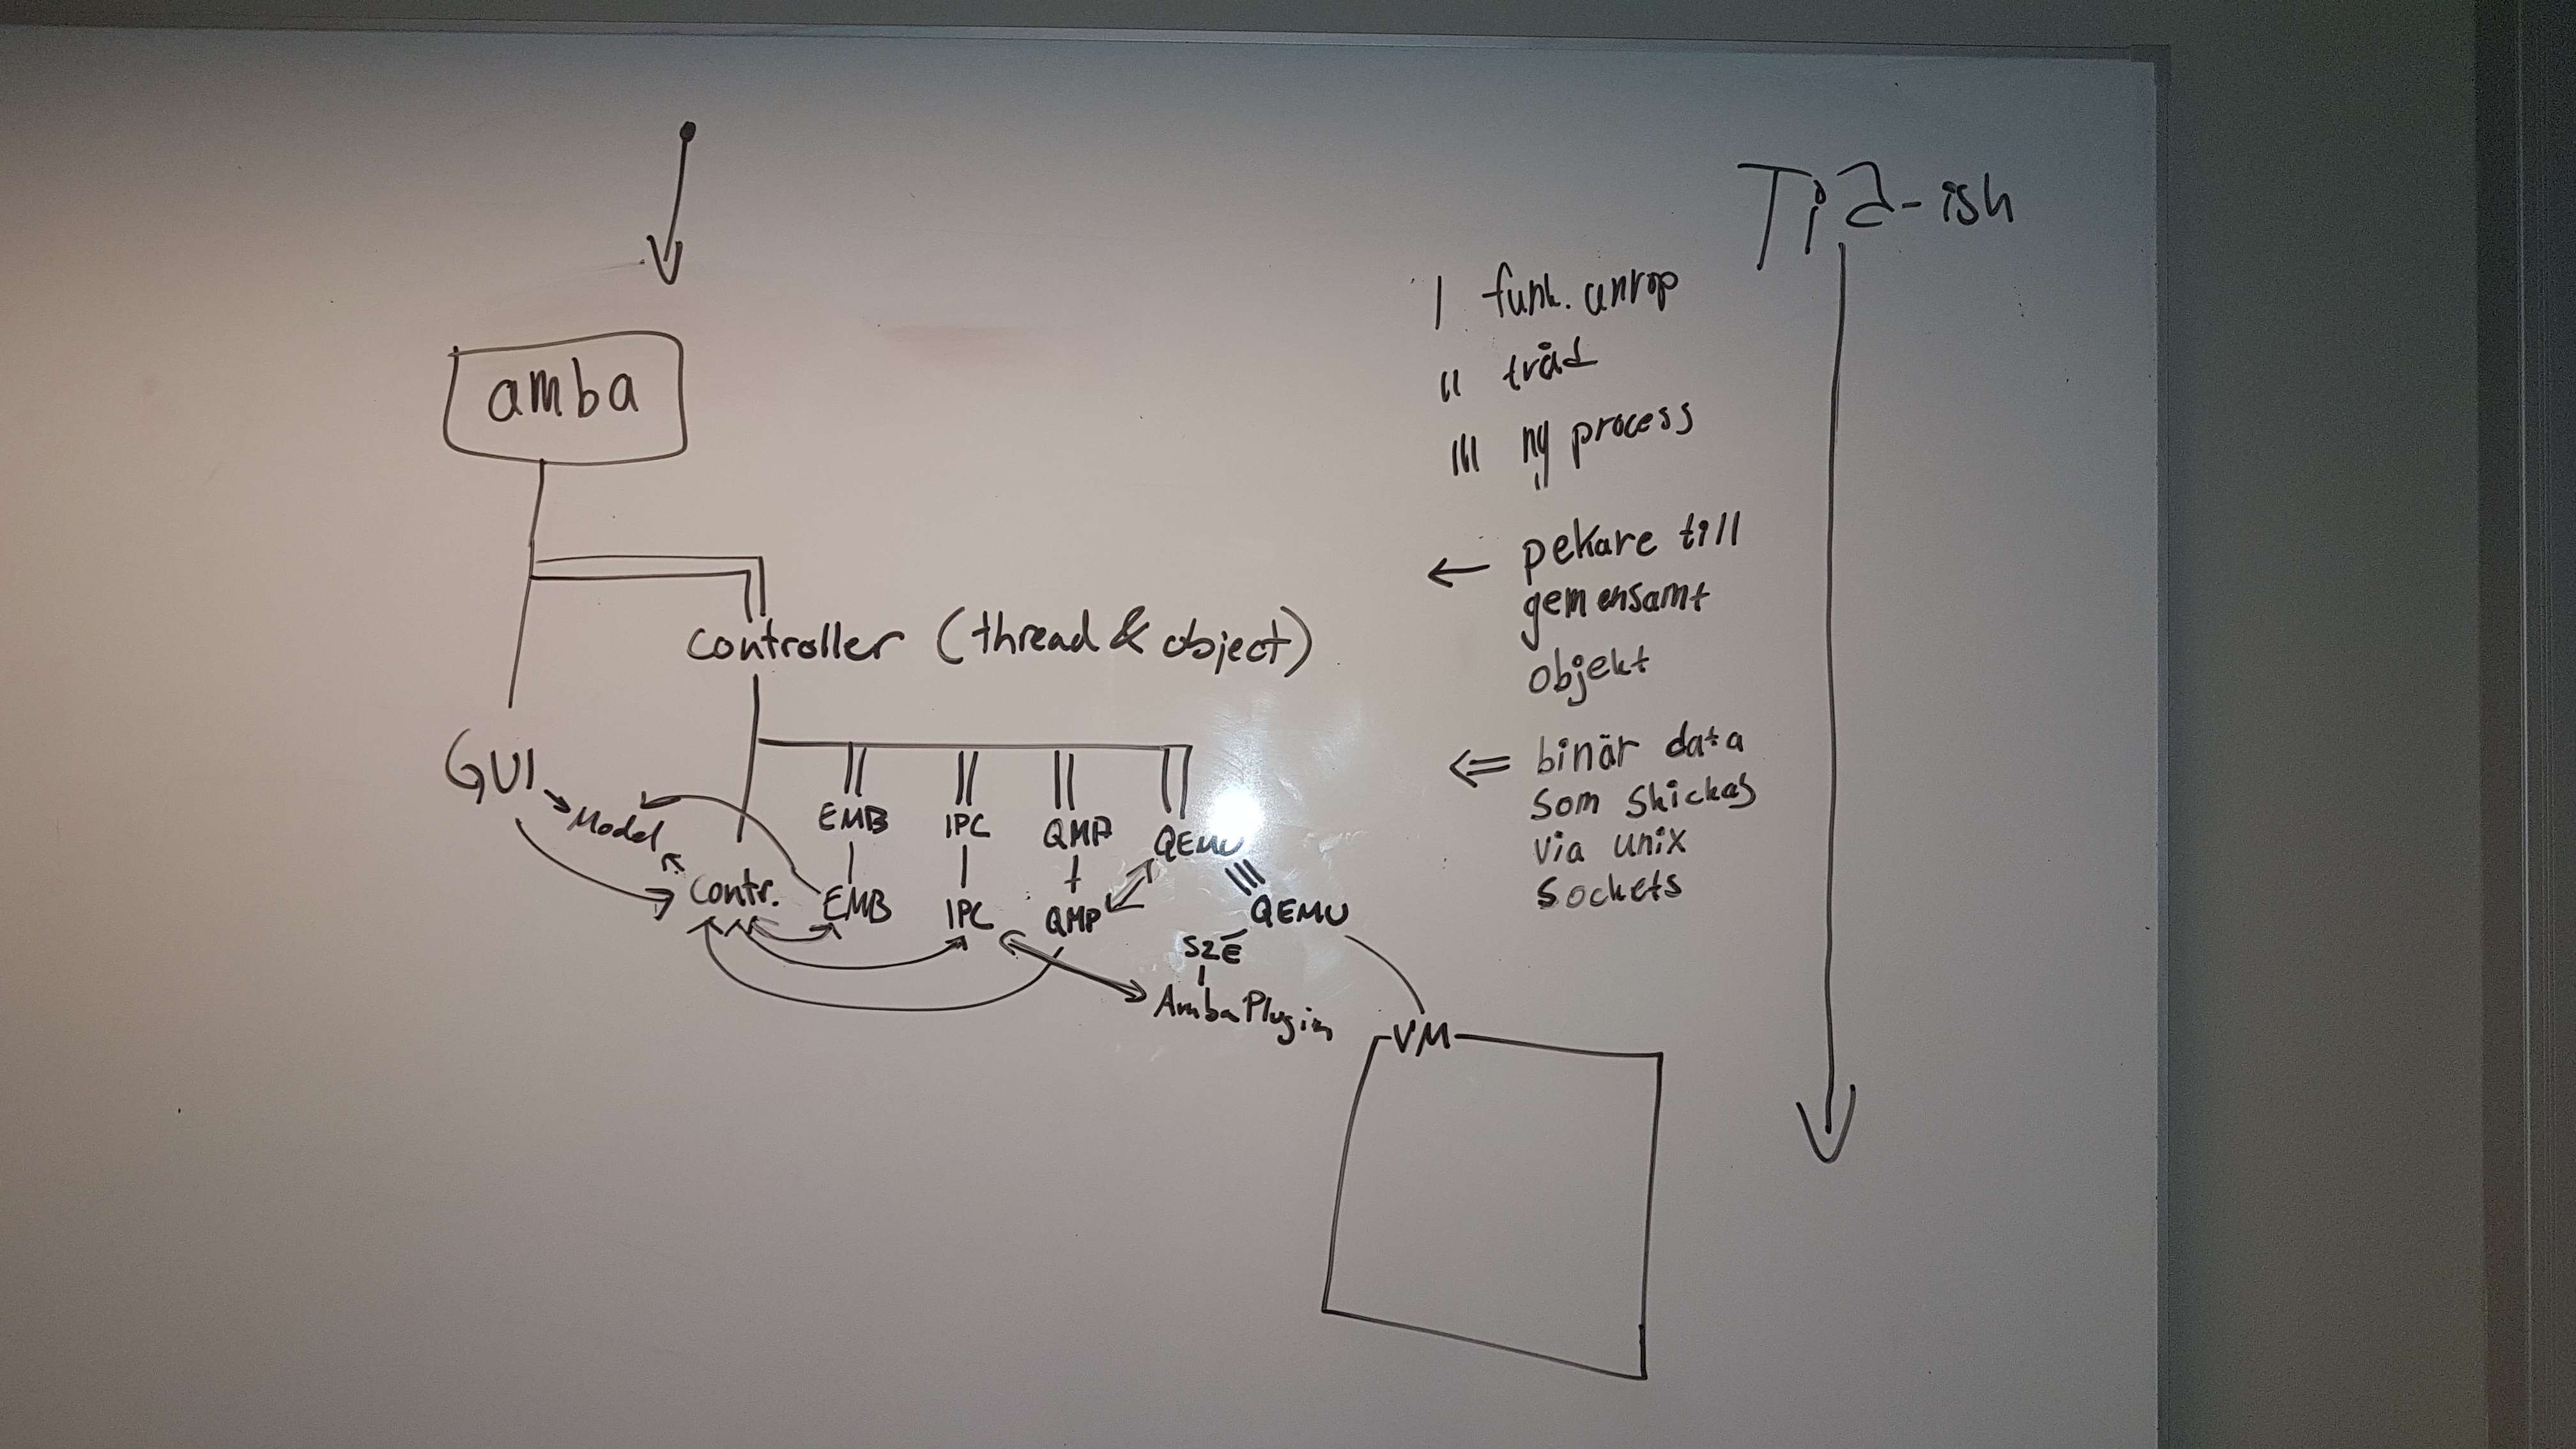
\includegraphics[width=\textwidth]{figures/arkitektur.jpg}
    \caption{[PLACEHOLDER] Systemöversikt över AMBA}\label{fig:arkitektur}
\end{figure}

%

AMBA ska betraktas som ett system bestående av ett flertalet subsystem som
kommunicerar med varandra med delade objekt eller unix socklar. Systemet tar
som indata en configurationsfil som bland annat specificerar sökvägen till
binären som ska analyseras samt inställningar till S2E. Utdatan är en
interaktiv graf baserad på symboliska uttryck som baseras på binärens maskinkod.
Grafen ger en visualisering över vilka möjliga vägar som exekveringen kan ta när
binären körs på en maskin. En översikt av systemets arkitektur finns i
figur~\ref{fig:arkitektur}. Med hjälp av inställningarna från
konfigurationsfilen startas sedan QEMU och \stoe{} med vårt \stoe{} plugin
AmbaPlugin. Ett operativsystem och binären laddas in och börjar exekveras.
\stoe{} anropar callbackfunktioner definierade i AmbaPlugin, vilka är tillagda i
utvalda \stoe{} hooks, som sedan uppdaterar vyn i vislualiseringen.

\section{Huvudprocess}

% Outline
% 1. Läser in en Recipe fil. (insällningar till s2e)
% (optional) 2. Startar GUI
% 3. Spawnar controller thread (gui gör det om man kör med GUI, annars amba direkt)
% 4. Controller spawnar QEMU (S2E); QMP listener (kommunikation mellan
%     controller och QEMU); IPC mekanism mellan libamba och controller; och
%     Embedder som layoutar en 2D graph för visualisering givet en CFG.

\subsection{Uppstart}

TODO

\subsection{GUI}

AMBA-processen använder immediate-mode-gui-biblioteket egui~\cite{egui} för att
rita sitt gränssnitt. Detta innebär att hela fönstret ritas om varje bildruta.
Processen samlar kantinformation som AmbaPlugin skickar och bygger de tre
graferna nämnda tidigare.

\section{\stoe{}}

\stoe{} använder sig av en modifierad QEMU instans för exekvering av olika
binärer och har en modulär arkitektur bestående av plugin som möjliggör analys
av binärer. Plugin har möjlighet att följa \stoe{}:s exekvering och undersöka
egenskaper för att spåra och forma analyser~\cite{Chipounov12}.

Konceptuellt består ett S2E plugin av ett tillstånd och en initieringsfuktion.
Tillståndet ärvs från ett kärn-plugin som innehåller information om bl.a.\
programtillstånd, symbolisk exekveringstillstånd och information om andra
plugin. Tillståndet kan utökas för att samla information, kontrollera egenskaper
och utföra binäranalys. Initieringsfunktionen består av tillståndsinitiering och
registrering av callbacks till olika hooks som tillgängligörs av antingen S2E:s
kärn-plugin eller andra plugin. Dessa callbacks anropas under exekvering när
motsvarande villkor för en hook uppfylls.

AmbaPlugin är ett S2E plugin som har utvecklats för att samla information under
exekvering av en binär ämnat för att visualisera exekveringen i AMBA.\@

\subsection{AmbaPlugin}

AmbaPlugin registrerar callbacks för ett antal hooks bland vilka
\texttt{onStateFork} och \texttt{onBlockStart}. När dessa hooks aktiveras
samlas information om S2E:s state id, generation för ett block i fallet av
självmodifierande kod, uttrycket för villkoret för att programexekveringen ska
nå denna state och ett id som utdelas till olika states. Utifrån detta
framställs kantinformation för CFG och Symbolisk state graf som kontinuerligt
skickas över IPC till GUI processen. Även annan information om varje nod i de
olika graferna samlas och skickas över IPC till GUI processen. Denna iterativa
informationsuppdateringen är tänkt att kommunicera framsteg till användaren
eftersom exekveringen kan ta lång tid beroende på den binär som analyseras.

\subsection{Packetering i pakethanteraren Nix}

S2E är ett komplicerat system och består av bland annat QEMU och behöver mycket
konfiguration för att sätta % upp en miljö för symbolisk exekvering. Verktyget
\textit{s2e-env} har tidigare utvecklats för att underlätta många steg som
skapandet av gäst-VM-avbild~\cite{s2e_website_s2eenv}. \textit{s2e-env} antar
däremot \textit{Ubuntu 18.04 LTS 64-bit OS} som värd för att kunna hämta rätt
beroenden~\cite{s2eenv_github}. Detta % har varit en svåröverkomlig krav för
utvecklandet av AMBA och därför har en nix-miljö framställts för att hantera och
bygga alla beroenden som krävs för att bygga och köra S2E med QEMU.

Nix-miljön har framställts för utveckling av AMBA och är inte lämplig för
upstreaming till \textit{s2e-env} i nuvarande form men kan vara möjligt efter
utökningar och modifieringar.

\section{Grafbehandling}

Huvudprocessen tar emot en ström av kanter representerade som ordnade par av
nodmetadata, där en mottagandet av en kant innebär att den kanten precis
bevandrats. Olika symboliska tillstånd har olika noder, vilket innebär att denna
kantströmmen innehåller all information som huvudprocessen behöver.

Nya noder placeras i en hashtabell och får ett sekventiellt allokerat id. Detta
id används sedan för att identifiera noden i olika representationer av grafen.
Grafen representeras med en grannlista för linjegrafskompression och nedbrytning
i starkt ansluta komponenter och med en kantlista för nodutplacering genom
kraftsimulation, och i båda dessa sammanhang är det praktiskt att noder
representeras som registerstora tal.

\subsection{Linjegrafskompression}

AMBA presenterar både en komprimerad och en okomprimerad graf för användaren.
Grafen komprimeras genom kantkontraktion av alla kanter anslutna till en nod av
ingrad exakt ett och utgrad exakt ett. Detta är ekvivalent med att se alla par
av grundblock som alltid förekommer efter varandra som ett enda grundblock.
Detta ger komprimerade grundblock som kan spänna flera funktioner och dynamiskt
länkade bibliotek.

Grafkompressionen sker online, alltså genom en datastruktur som samtidigt
tillåter tilläggning av kanter i grafen och kan svara på frågor om vilka kanter
som kommer in samt går ut från en (komprimerad) nod. Detta implementeras genom
att lagra både en komprimerad och okomprimerad graf. En pekare till den
okomprimerade grafen delas ut till läsare. När en kant ska läggas till
kontrolleras först om denna redan finns i den okomprimerade grafen. Om inte
återställs de kantkontraktioner som skapat de komprimerade noder som innehåller
kantens ändnoder. Därefter läggs kanten till och grafen komprimeras lokalt.
Tidskomplexiteten för kanttilläggningar är då lika med summan av kardinaliteten
på de komprimerade noder som innehåller kantens slutnoder. Detta är kvadratiskt
i värstafallet en enda linjegraf men fungerar i praktiken då
kontrollflödesgrafen inte innehåller långa linjegrafer. Författarna är medvetna
om att en fullt linjär algoritm existerar.

\subsection{Starkt anslutna komponenter}

AMBA kan färglägga noder i de komprimerade och ickekomprimerade
kontrollflödesgraferna efter deras så kallade starkt anslutna komponent (jrf.\
eng.\ strongly connected component). En riktad grafs starkt anslutna komponenter
är ekvivalensklasserna under relationen att ett par av noder är både nedströms
och uppströms ifrån varandra. Den starkt anslutna komponenten som en nod $V$
tillhör är alltså mängden av de noder som både kan nå $V$ och som kan nås av
$V$.

AMBA bryter ned grafer i deras starkt anslutna komponenter med Tarjans
algoritm~\cite{tarjan}. Tarjans algoritm bygger på en rekursiv DFS, och AMBA
hanterar dess linjära stackdjup genom att köra algoritmen på en tråd med en
tillräckligt stor stack.

\subsection{Nodutplacering genom kraftsimulation}

Nodutplaceringen styrs av en attraktionskraft mellan kopplade noder som är
proportionelig mot $D^{1.2}$ på avståndet $D$, en repulsionskraft mellan alla
par av noder som är proportionelig mot $\frac{D}{1+D^3}$ och en
gravitationskraft som påverkar alla noder utom rotnoden i negativ y-led.

Hastighet och position integreras med Euler framåt, men magnituden på
hastigheten ändras dessutom direkt: den ökas exponentiellt när accelerationen
och hastigheten är likriktade och minskas exponentiellt annars. Detta ger
snabbare konvergens. Positionen kan även uppdateras med uniformt brus om
användaren har ställt in detta som nollskilt.

Slutligen gäller tvång som placerar rotnoden i origo och masscentrum på axeln
vertikalt under. Därmed går exekvering framförallt uppifrån ned.

Den beräkningstunga delen av nodutplaceringen är beräkningen av
repulsionskraften. Naiv summation mellan varje par av noder tar $O(n^2)$ tid per
tidssteg eller $O(n^3)$ tid totalt under antagande att konvergens nås efter
linjärt många steg. Därför implementerar AMBA även Barnes-Hut
kraftberäkningsalgoritm på ett R-träd. Ett R-träd är ett balanserat binärt träd
av punktmängder där varje lövnod är en enskild punkt och varje grennod lagrar
begränsningslådan för punkterna den innehåller. AMBA bygger trädet genom att
rekursivt hugga den axel som är geometriskt längst och använder en parameter för
att bestämma vid kvot mellan lådstorlek och kraftavstånd där lådan anses
tillräckligt liten för att dess noder kan approximeras ligga i lådans
masscentrum. Barnes-Hut har en tidskomplexitet på $O(n\log n)$ per tidssteg
eller för oss $O(n^2\log n)$ totalt vilket möjliggör utplacering av större
grafer.
